\documentclass[aps,prl,twocolumn,10pt,superscriptaddress,nofootinbib,longbibliography,floatfix]{revtex4-2}

\usepackage{amsmath,amssymb,bm}
\usepackage{graphicx}
\usepackage{booktabs}
\usepackage[colorlinks=true,linkcolor=blue,citecolor=blue,urlcolor=blue]{hyperref}

\newcommand{\dd}{\mathrm{d}}
\newcommand{\Mzero}{M_0}
\newcommand{\chizero}{\chi_0}
\newcommand{\mbin}{m_{\mathrm{bin}}}
\newcommand{\ain}{a_{\mathrm{in}}}
\newcommand{\ein}{e_{\mathrm{in}}}
\newcommand{\aout}{a_{\mathrm{out}}}
\newcommand{\Izero}{I_0}
\newcommand{\RH}{R_{\mathrm{H}}}
\newcommand{\fH}{f_{\mathrm{H}}}
\newcommand{\epsGR}{\epsilon_{\mathrm{GR}}}
\newcommand{\tZKL}{t_{\mathrm{ZKL}}}
\newcommand{\rPsifour}{r\Psi_4}

\setlength{\textfloatsep}{8pt plus 2pt minus 2pt}
\setlength{\dbltextfloatsep}{9pt plus 2pt minus 2pt}

\begin{document}

\title{Relativistic Zeipel--Kozai--Lidov Oscillations of Compact Binaries\texorpdfstring{\\}{ }around Supermassive Black Holes in Full Numerical Relativity}

\author{Haiyang Wang}
\email{haiyangw@princeton.edu}
\affiliation{Department of Astrophysical Sciences, Princeton University, Princeton, NJ 08544, USA}

\date{\today}

\begin{abstract}
Stellar-mass black-hole binaries embedded in active galactic nucleus disks form hierarchical triples with a central supermassive black hole. Tidal torques from the central black hole drive Zeipel--Kozai--Lidov eccentricity and inclination cycles that accelerate compact-binary inspirals and imprint secular modulations onto gravitational radiation. Secular post-Newtonian approximations break down once the outer orbit probes strong spacetime curvature, spin-induced frame dragging twists the orbital planes, and inner pericenter separations enter the relativistic merger regime. We formulate and calibrate a full three-plus-one numerical relativity framework evolving a central spinning puncture coupled to two self-gravitating compact particles through fourth-order implicit Gauss--Legendre particle transport, piecewise-cubic spline deposition, and conservative metric filtering. A local Fermi-normal harmonic coordinate mapping removes spurious gauge eccentricity on initialization, while separation-adaptive mesh refinement across nested grid levels paired with tracker-normalized Gamma-driver shift damping and per-cycle matter coupling eliminates late-time mesh drag across eccentric Zeipel--Kozai--Lidov pericenters toward compact-binary merger.
\end{abstract}

\maketitle

\section{Introduction}
Stellar-mass binary black holes trapped inside active galactic nucleus (AGN) migration traps naturally assemble into compact hierarchical triples alongside the central supermassive black hole (SMBH) of mass $\Mzero$ and dimensionless spin $\chizero$ \cite{Hoang:2018,Liu:2018,Liu:2019}. When the inner orbital plane of the stellar-mass pair is strongly inclined relative to the outer orbit about the SMBH, secular Newtonian tidal torques exchange eccentricity $\ein$ and mutual inclination $I$ through the Zeipel--Kozai--Lidov (ZKL) mechanism \cite{vonZeipel:1910,Kozai:1962,Lidov:1962,Naoz:2016}. Eccentricity surges compress pericenter passages, radiate intense gravitational-wave bursts \cite{Blaes:2002,Randall:2018}, and alter binary-EMRI phasing signatures targeted by spaceborne detectors.

Orbit-averaged secular perturbation theory captures weak-field hierarchical triples well, yet becomes unreliable for binary EMRIs orbiting close to the SMBH horizon. Three relativistic effects compete directly within a few dozen gravitational radii of the SMBH: general-relativistic apsidal precession inside the binary can quench quadrupole growth \cite{Blaes:2002,Liu:2015}; frame dragging from a spinning Kerr SMBH torques both orbital angular momenta and shifts secular resonances; and strong tidal curvature couples inner orbital eccentricity directly into outgoing gravitational radiation \cite{Cardoso:2026}. Capturing the coupled spacetime and few-body dynamics free of orbit-averaging assumptions demands solving the full Einstein field equations alongside self-gravitating relativistic trajectories.

In this Letter, we present a systematic numerical-relativity investigation targeting binary-EMRI ZKL dynamics around both Schwarzschild and rapidly spinning Kerr SMBHs using high-order relativistic particle-in-cell coupling on a Z4c spacetime background \cite{Bona:2003fj,Hilditch:2012fp,Zhu:2024utz,2026ApJS..283...27S,Wu:2026nrpic}. We establish the initial-data coordinate mapping required to place bound binaries inside strong-field background potentials, validate the astrophysical parameter space across inclination, precession quenching, spin coupling, and octupole asymmetry using a post-Newtonian (PN) scout, and deploy a compact separation-adaptive mesh hierarchy engineered for zero-drag secular integration through compact-binary merger with high-cadence Weyl waveform diagnostics.

\section{Relativistic Triple Formulation}
We model the AGN binary-EMRI triple as one central moving-puncture SMBH \cite{Campanelli:2005dd,Baker:2005vv,Bowen:1980yu} of ADM mass $\Mzero$ and spin vector $\bm{S}_0 = \Mzero^2 \chizero \hat{\bm{z}}$, orbited at semimajor axis $\aout$ by two gravitating massive particles of individual masses $m_1$ and $m_2$ ($\mbin = m_1 + m_2 \ll \Mzero$) and initial inner semimajor axis $\ain$. Long-term dynamical stability against three-body tidal ionization requires that the binary reside safely inside its Hill radius $\RH \equiv \aout [\mbin/(3\Mzero)]^{1/3}$, parameterized by the dimensionless Hill filling fraction $\fH \equiv \ain / \RH$.

Secular evolution of the inner binary is governed by the ratio between general-relativistic pericenter precession and the quadrupole ZKL torque rate $\tZKL^{-1}$, yielding the relativistic quenching ratio \cite{Blaes:2002,Liu:2015}
\begin{equation}
  \epsGR = \frac{3 \mbin^2 \aout^3}{\Mzero \ain^4},
\end{equation}
assuming a circular outer orbit of period $P_{\mathrm{out}}$ and inner period $P_{\mathrm{in}}$, with characteristic timescale $\tZKL \approx (P_{\mathrm{out}}^2 / P_{\mathrm{in}})(\Mzero + \mbin)/(2\Mzero)$. In our full numerical relativity evolutions, spacetime geometry follows the conformal Z4c formulation \cite{Hilditch:2012fp,Zhu:2024utz} in moving-puncture gauge with increased constraint damping ($\kappa_1 = 0.50$) and tracker-normalized Gamma-driver shift damping ($\eta_0 = 0.07$), while the two stellar-mass black hole particles advance through fourth-order implicit Gauss--Legendre symplectic time integration \cite{SanzSerna:1988,Wu:2026nrpic} paired with per-cycle matter coupling, quadratic metric time interpolation, quintic metric reconstruction, piecewise-cubic spline deposition, and split metric-conservative source filtering.

Direct naive initialization of Newtonian Keplerian binary velocities in global isotropic or harmonic coordinates fails in the strong field near $\Mzero$. At an outer separation $\aout$, gravitational redshift and spatial conformal contraction suppress the coordinate gravitational acceleration between $m_1$ and $m_2$ relative to local proper separation, inducing spurious orbital eccentricity of order the background potential $\Phi_0 = \Mzero/\aout$ within a single inner period. We construct consistent triple initial data via the local-frame harmonic transformation linking proper Fermi-normal elements $(\bm{R}_{\mathrm{loc}}, \bm{U}_{\mathrm{loc}})$ in the freely falling binary frame (moving at outer center-of-mass velocity $\bm{V}_{\mathrm{com}}$) to global harmonic coordinates $(\bm{r}_{\mathrm{harm}}, \bm{u}_{\mathrm{harm}})$:
\begin{align}
  \bm{r}_{\mathrm{harm}} &= (1 - \Phi_0)\bm{R}_{\mathrm{loc}} - \tfrac{1}{2}(\bm{R}_{\mathrm{loc}}\cdot\bm{V}_{\mathrm{com}})\bm{V}_{\mathrm{com}}, \\
  \bm{u}_{\mathrm{harm}} &= \left(1 - \tfrac{5}{2}\Phi_0 - \tfrac{1}{2}V_{\mathrm{com}}^2\right)\bm{U}_{\mathrm{loc}} - \tfrac{1}{2}(\bm{U}_{\mathrm{loc}}\cdot\bm{V}_{\mathrm{com}})\bm{V}_{\mathrm{com}}.
\end{align}
For full numerical-relativity initial slices, particle coordinates, covariant momenta, companion Gaussian conformal wells matching the smoothed deposition width, self-binding bare-mass compensation, and the balancing SMBH puncture momentum feed into the elliptic conformal-and-momentum constraint solver prior to Z4c evolution, maintaining physical constraint satisfaction without transient eccentricity bursts or mesh self-force drift.

\section{Secular Excitation, Quenching, and Spin Coupling}
Before launching production three-plus-one numerical-relativity runs, we calibrate a four-suite parameter matrix at fixed SMBH mass $\Mzero$ and near-circular initial inner eccentricity $e_0$ using our Fermi-transformed Einstein--Infeld--Hoffmann plus Kerr Lense--Thirring scout integrator. Every trajectory remains bound inside the Hill sphere over multiple outer orbital periods, isolating four distinct dynamical regimes illustrated in Fig.~\ref{fig:zkl_scout}.

\begin{figure*}[t]
  \centering
  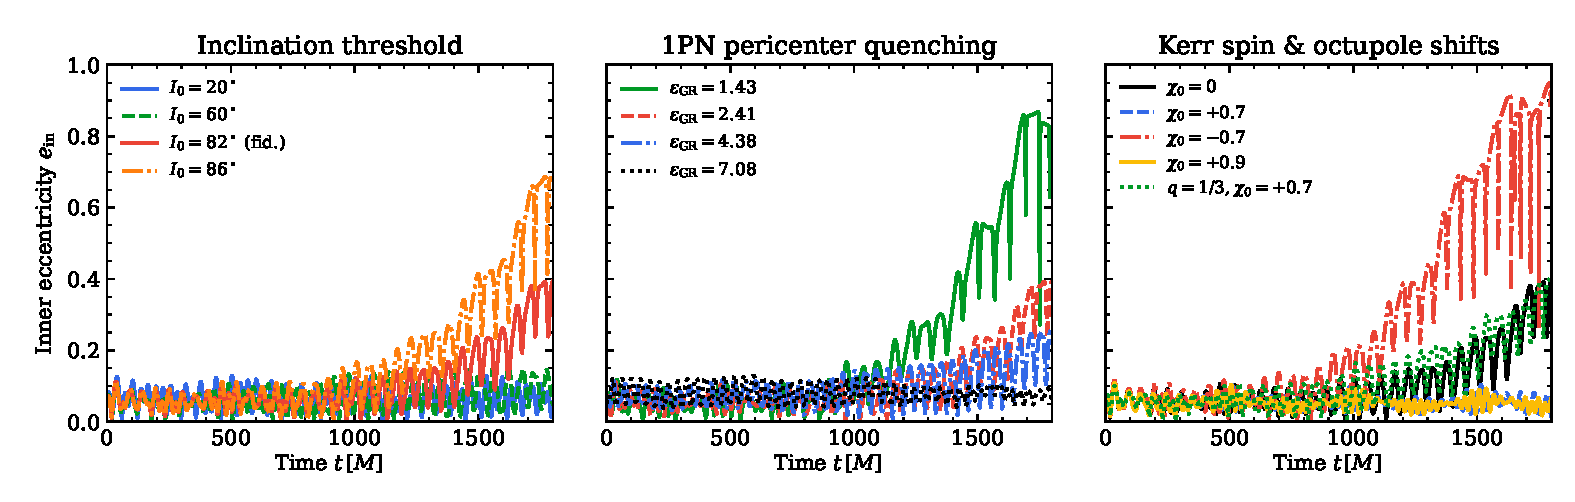
\includegraphics[width=\textwidth]{figures/fig_zkl_scout.pdf}
  \caption{Calibrated relativistic inner-eccentricity trajectories across four regimes at fixed binary mass. Left: inclination threshold separating flat subcritical evolution from steep quadrupole growth. Center: monotonic pericenter quenching with rising $\epsGR$. Right: prograde Kerr suppression vs.\ retrograde resonance and octupole revival.}
  \label{fig:zkl_scout}
\end{figure*}

First, varying the initial mutual inclination $\Izero$ at fixed $\epsGR$ maps the relativistic inclination threshold: orbits below or modestly above the Newtonian critical angle remain near-circular, whereas highly inclined triples undergo rapid eccentricity surges once quadrupole torques overcome relativistic apsidal drift. Second, varying $\ain$ at fixed $\mbin$ sweeps $\epsGR$ while preserving a common stellar-mass ratio. This constant-mass sweep isolates pure pericenter precession quenching, monotonically suppressing peak eccentricity from strong high-eccentricity cycles down to weak bounded librations. Third, reversing the SMBH Kerr spin $\chizero$ separates two strongly asymmetric branches at identical orbital geometry: prograde spins suppress eccentricity growth through additive nodal precession, while a retrograde spinning SMBH shifts the secular resonance into deep amplification approaching merger pericenters. Fourth, breaking mass equality to an unequal mass ratio re-excites octupole-driven eccentricity modulation \cite{Naoz:2013,Liu:2015} even when prograde frame dragging suppresses the equal-mass channel.

\textit{[PENDING FULL-NR RUNS: Upon completion of the queued production evolutions, full three-plus-one numerical-relativity inner-binary tracks transformed via the local-frame harmonic inversion will be overlaid against these post-Newtonian curves in Fig.~2 to quantify non-perturbative strong-field departures, orbital energy loss, and apparent-horizon mass and spin evolution.]}

\section{Gravitational-Wave Signatures and Conclusions}
Probing hierarchical ZKL oscillations through full numerical relativity unlocks waveform observables inaccessible to orbit-averaged calculations. During high-eccentricity phases driven either by steep inclination or by retrograde Kerr spin-orbit resonance, pericenter compression steepens instantaneous orbital frequency and radiates periodic bursts of quadrupolar radiation superposed on the outer orbital modulation. To resolve both inner-binary pericenter harmonics and outer-orbital Doppler shifts cleanly, outgoing Newman--Penrose scalars $\rPsifour$ are extracted across concentric spherical shells at fivefold higher temporal cadence than standard single-black-hole evolutions \cite{Bishop:2016lgv,Reisswig:2010di}.

\textit{[PENDING FULL-NR RUNS: Extracted multipolar waveforms $\rPsifour$, integrated strain harmonics across pericenter bursts, and nonlinear coupling between SMBH frame dragging and high-eccentricity gravitational-wave emission will populate this section and Fig.~3 once the queued production runs finish.]}

In summary, combining a moving-puncture SMBH with high-order implicit gravitating binary particles and a Fermi-transformed initial-data pipeline establishes an affordable route to self-consistent ZKL dynamics in full general relativity. The calibrated four-suite parameter map identifies exact dynamical regimes where three-plus-one evolutions directly test relativistic quenching, retrograde spin-orbit amplification, and octupole eccentricity bursts relevant to AGN LISA sources.

\appendix

\section{Numerical Architecture and Simulation Catalog}
To execute multi-cycle ZKL evolutions through pericenter compression and merger while keeping the central puncture resolved across thousands of gravitational times, we construct a separation-adaptive mesh hierarchy built from $16^3$ cell blocks spanning $[-64, 64]^3 M$. Coarse asymptotic zones host multipole Robin multigrid boundaries during initial-data constraint solving, a static radial tracker encloses the wave-extraction region ($r \le 24\,M$ at $L_1 = 1.0\,M$) while concentric spheres at $r = 22$, $30$, and $38\,M$ sample outgoing $\rPsifour$ at cadence $\Delta t_{\Psi} = 0.1\,M$, a spin-adaptive central core refines down to $M/32$ on $[-0.85, 0.85]^3 M$ for $|\chizero| \le 0.7$ and $M/64$ on $[-0.48, 0.48]^3 M$ for $\chizero = +0.9$ to maintain at least $32$ cells across the evolved apparent-horizon diameter, and custom binary-separation refinement (\texttt{amr\_dyn}) dynamically nests the comoving binary across levels $L_5$--$L_8$ ($M/16$ to $M/128$) as separation contracts. Pairing six-pass piecewise-cubic spline filtering ($\sigma_{\mathrm{eff}} = 0.1141\,M$ at $L_5$) and per-cycle matter coupling with $\kappa_1 = 0.50$ and tracker-normalized shift damping ($\eta_0 = 0.07$) suppresses artificial secular angular-momentum drift to $|d\ln L_z/dt| = 3.89\times 10^{-5}\,M^{-1}$ using only $596$--$834$ cell blocks. Calibration runs verified close-encounter refinement ($d_{\min} = 0.0555\,M$), horizon stability ($|\Delta M/M_0| = 7.3\times 10^{-5}$), and metric-conservative conservation prior to launching the production suite in Table~\ref{tab:runs}, anchored by $M_0 = 1.0$, $\aout = 15.0\,M$, and $e_0 = 0.05$.

\begin{table*}[t]
  \caption{Production parameter matrix for the full three-plus-one numerical-relativity ZKL suite ($M_0 = 1.0$, $a_{\mathrm{out}} = 15.0\,M$, $e_0 = 0.05$), showing particle masses ($m_1, m_2$), inner semimajor axis $a_{\mathrm{in}}$, inclination $I_0$, SMBH spin $\chi_0$, Hill filling ratio $f_{\mathrm{H}}$, GR quenching ratio $\epsilon_{\mathrm{GR}}$, ZKL timescale $t_{\mathrm{ZKL}}$, and calibrated 1PN peak eccentricity $e_{\max}^{\mathrm{1PN}}$ and minimum separation $r_{\min}$ over $t \le 1800\,M$.}
  \label{tab:runs}
  \begin{ruledtabular}
  \begin{tabular}{llcccccccc}
    Run ID & Suite & $m_1, m_2\,[M_0]$ & $a_{\mathrm{in}}\,[M]$ & $I_0\,[\mathrm{deg}]$ & $\chi_0$ & $f_{\mathrm{H}}$ & $\epsilon_{\mathrm{GR}}$ & $t_{\mathrm{ZKL}}\,[M]$ & $e_{\max}^{\mathrm{1PN}}\,(r_{\min}/M)$ \\
    \hline
    \texttt{I20\_subcrit}  & Inclination & $0.004, 0.004$ & $0.72$ & $20$ & $0.0$  & $0.346$ & $2.411$ & $1552.3$ & $0.128\,(0.703)$ \\
    \texttt{I60\_mild}     & Inclination & $0.004, 0.004$ & $0.72$ & $60$ & $0.0$  & $0.346$ & $2.411$ & $1552.3$ & $0.158\,(0.670)$ \\
    \texttt{FID\_I82\_chi0}& Fiducial    & $0.004, 0.004$ & $0.72$ & $82$ & $0.0$  & $0.346$ & $2.411$ & $1552.3$ & $0.394\,(0.467)$ \\
    \texttt{I86\_high}     & Inclination & $0.004, 0.004$ & $0.72$ & $86$ & $0.0$  & $0.346$ & $2.411$ & $1552.3$ & $0.687\,(0.253)$ \\
    \texttt{GR\_low\_a082} & GR quench   & $0.004, 0.004$ & $0.82$ & $82$ & $0.0$  & $0.394$ & $1.433$ & $1277.2$ & $0.868\,(0.113)$ \\
    \texttt{GR\_mid\_a062} & GR quench   & $0.004, 0.004$ & $0.62$ & $82$ & $0.0$  & $0.298$ & $4.385$ & $1942.6$ & $0.254\,(0.515)$ \\
    \texttt{GR\_high\_a055}& GR quench   & $0.004, 0.004$ & $0.55$ & $82$ & $0.0$  & $0.264$ & $7.081$ & $2325.0$ & $0.130\,(0.559)$ \\
    \texttt{SPIN\_p07}     & Kerr spin   & $0.004, 0.004$ & $0.72$ & $82$ & $+0.7$ & $0.346$ & $2.411$ & $1552.3$ & $0.109\,(0.714)$ \\
    \texttt{SPIN\_m07}     & Kerr spin   & $0.004, 0.004$ & $0.72$ & $82$ & $-0.7$ & $0.346$ & $2.411$ & $1552.3$ & $0.948\,(0.074)$ \\
    \texttt{SPIN\_p09}     & Kerr spin   & $0.004, 0.004$ & $0.72$ & $82$ & $+0.9$ & $0.346$ & $2.411$ & $1552.3$ & $0.109\,(0.716)$ \\
    \texttt{OCT\_q3\_I80}  & Octupole    & $0.006, 0.002$ & $0.72$ & $80$ & $+0.7$ & $0.346$ & $2.411$ & $1552.3$ & $0.412\,(0.460)$ \\
  \end{tabular}
  \end{ruledtabular}
\end{table*}

\bibliography{references}

\end{document}
